\documentclass[table, 12pt]{article}
\usepackage{graphicx}
\usepackage[T1]{fontenc}
\usepackage{tocloft}
\usepackage{todonotes}
\usepackage{caption}
\usepackage{hyperref}
\usepackage{booktabs}
\usepackage{listings}
\usepackage{pdfpages}
\usepackage{pdflscape}
\usepackage{textpos}
\usepackage{scrhack}
\usepackage{xcolor}
\usepackage{float}
\usepackage{longtable}
\usepackage{enumerate}
\usepackage{tasks}
\usepackage{tabularx}
\usepackage{titlesec}
\usepackage{listing}
\usepackage{graphicx}
\usepackage{subcaption}
\usepackage[export]{adjustbox}

\hyphenation{group-ed}

\titleformat{\paragraph}
{\normalfont\normalsize\bfseries}{\theparagraph}{1em}{}
\titlespacing*{\paragraph}
{0pt}{3.25ex plus 1ex minus .2ex}{1.5ex plus .2ex}
\begin{document}
\begin{titlepage}
    \centering
    {\scshape\large AY 2022/2023 \par}
    \vfill
    
\includegraphics[width=100pt]{assets/logo_polimi}\par\vspace{1cm}
    {\scshape\LARGE Politecnico di Milano \par}
    \vspace{1.5cm}
    {\huge\bfseries Acceptance Testing Document \par}
    \vspace{2cm}
    {\Large {Francesco Dubini\quad Marcello De Salvo\quad\par Riccardo Grossoni}\par}
    \vfill
    {\large Professor\par
        Elisabetta \textsc{Di Nitto}}
    \vfill
    {\large \textbf{Version 1.0} \\ \today \par}
\end{titlepage}
\hypersetup{%
    pdfborder = {0 0 0}
}
\thispagestyle{plain}
\pagenumbering{gobble}
\mbox{}
\newpage
\pagenumbering{roman}
\tableofcontents
\newpage
\pagenumbering{arabic}

\section{Tested Project}
\begin{itemize}
    \item \textbf{Authors}
    \\Giovanni De Lucia, Lorenzo Battiston, Matteo Currò
    \item \textbf{Repository URL}\\ \underline{\url{https://github.com/gio-del/BattistonDeLuciaCurro-swe2}}
    \item \textbf{Documents considered}\begin{itemize}
              \item RASD: Requirements Analysis Specification Document;
              \item DD: Design Document;
              \item ITD: Implementation and Testing Document;
          \end{itemize}
\end{itemize}
\newpage

\section{Installation}
Thanks to the provided Dockerfile, the project can be easily installed and run, so the installation was not a problem. Furthermore the github wiki contains detailed information on 
pre-made accounts for testing, and shows how to get around the inital 2FA at registration.

\section{Acceptance Test Cases}

\subsection{Sign up \& Log in}
\begin{itemize}
    \item[\textit{i.}] \textbf{Goal} User authentication (CPMS and eMSP)
    \item[\textit{ii.}] \textbf{Test Cases}
    \begin{itemize}
        \item[(a)] Register with valid credentials
        \item[(b)] Register with invalid credentials
        \item[(c)] Register with a phone number or email already in use
        \item[(d)] Login with correct credentials
        \item[(e)] Login with wrong credentials
    \end{itemize} 
    \item[\textit{iii.}] \textbf{Test Results}
    \begin{itemize}
        \item[(a)] The registration is successful and the user is redirected to the login page
        \item[(b)] The registration fails and the correct error message is shown
        \item[(c)] The registration fails and the correct error message is shown
        \item[(d)] The login is successful and the user is redirected to the home page
        \item[(e)] The login fails and the correct error message is shown
    \end{itemize} 
    \item[\textit{iv.}] \textbf{Issues}    
    \begin{itemize}
        \item Nothing to report
    \end{itemize} 
\end{itemize}
\subsection{Charging Stations Map}
\begin{itemize}
    \item[\textit{i.}] \textbf{Goal} Visualize Charging stations data
    \item[\textit{ii.}] \textbf{Test Cases}
    \begin{itemize}
        \item[(a)] See the map of charging stations in the home page
        \item[(b)] See the status of the charging stations
    \end{itemize}
    \item[\textit{iii.}] \textbf{Test Results}
    \begin{itemize}
        \item[(a)] The map correctly displays the charging stations
        \item[(b)] Clicking a charging station correctly displays the information
    \end{itemize} 
    \item[\textit{iv.}] \textbf{Issues}    
    \begin{itemize}
        \item Nothing to report
    \end{itemize} 
\end{itemize}

\subsection{Book a charging station}
\begin{itemize}
    \item[\textit{i.}] \textbf{Goal} Book a charging station
    \item[\textit{ii.}] \textbf{Test Cases}
    \begin{itemize}
        \item[(a)] Book a charging station's socket for a valid time interval
        \item[(b)] Book a charging station's socket for an already booked time interval
        \item[(c)] Book a charging station's socket for a date in the past
        \item[(d)] Book a charging station's socket in a charging station without sockets
    \end{itemize} 
    \item[\textit{iii.}] \textbf{Test Results}
    \begin{itemize}
        \item[(a)] The Booking is correctly handled
        \item[(b)] The already booked time intervals are not shown as options
        \item[(c)] Past dates and hours are not shown as options
        \item[(d)] An exception error is thrown and not handled correctly
    \end{itemize}
    \newpage
    \item[\textit{iv.}] \textbf{Issues}    
    \begin{itemize}
        \item When a booking is made for the current time, e.g. if it is 10.03 AM and i book specifically for this time, the time invervals options become shifted by the minute amount for the rest of the day.\\
        In the case the booking spans between days this effect is propagated throughout all the next day. So if I book a charge from 23.58 to 01.58 all throughout the next day other users will only be able to book in the .28/.58 minutes.
        It would likely be more correct to round out the end time of bookings completely at the half hour mark or give complete freedom in terms of minutes.
        \item If "Book" is clicked in a station without sockets, an unhandled exception error is thrown.
    \end{itemize} 
\end{itemize}
\begin{figure}[H]
   \centering
    \includegraphics[scale=0.44, center]{assets/booking_shifted_time.jpg}
    \caption{booking shift bug - the half and hour marks are not displayed correctly}
    \label{fig: Booking_shift}
\end{figure}
\begin{figure}[H]
   \centering
    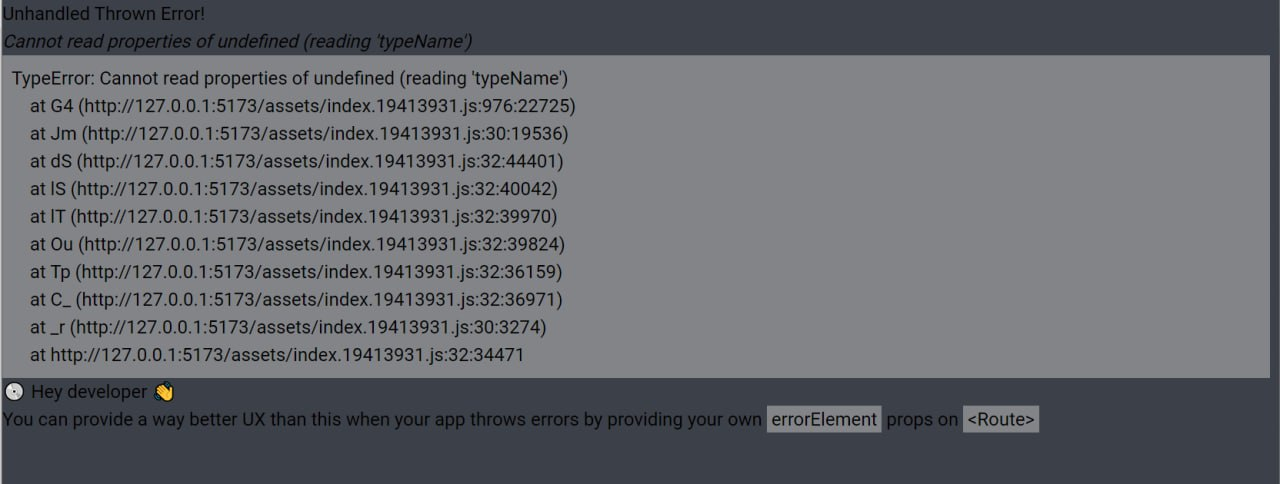
\includegraphics[scale=0.33, center]{assets/unhandled_booking_error.jpg}
    \caption{booking a socketless station - the error is not handled correctly server-side}
    \label{fig: Booking_socketless}
\end{figure}
\subsection{Start a charging session}
\begin{itemize}
    \item[\textit{i.}] \textbf{Goal} Start a charging session for a booked socket
    \item[\textit{ii.}] \textbf{Test Cases}
        \begin{itemize}
            \item[(a)] Start a charging session
            \item[(b)] Check if the socket becomes unavailable for other users
            \item[(c)] Insert negative values for the percentage of battery to be charged
        \end{itemize}
    \item[\textit{iii.}] \textbf{Test Results}
        \begin{itemize}
            \item[(a)] The charging session is correctly started
            \item[(b)] The socket is correctly marked as unavailable
            \item[(c)] The charging session is started but the negative values are not handled correctly
        \end{itemize}
    \item[\textit{iv.}] \textbf{Issues}
    \begin{itemize}
        \item If a negative value is inserted for the percentage of energy to be charged, the charging session is started but the negative values are not handled correctly since they gets displayed in the charging session page.
        \item You cannot stop a charging session manually, you have to wait for it to end.
        \item When clicking start for a charging session the page does not automatically redirect to the charging session page. It's not an error but we think that it should be implemented.
    \end{itemize} 
\end{itemize}

\subsection{CPO add special offers and rates}
\begin{itemize}
    \item[\textit{i.}] \textbf{Goal} Register a special offer for a charging station
    \item[\textit{ii.}] \textbf{Test Cases}
    \begin{itemize}
        \item[(a)] Register a special offer
        \item[(b)] Delete a special offer
        \item[(c)] Register a special offer with invalid values
        \item[(d)] Register a rate
        \item[(e)] Register a rate with invalid values
    \end{itemize}
    \item[\textit{iii.}] \textbf{Test Results}
    \begin{itemize}
        \item[(a)] The offer is registered correctly
        \item[(b)] The offer is deleted correctly
        \item[(c)] The offer is not registered, but no error message is shown
        \item[(d)] The rate is registered correctly
        \item[(e)] The rate is registered with negative values
    \end{itemize} 
    \item[\textit{iv.}] \textbf{Issues}    
    \begin{itemize}
        \item When trying to register an invalid offer (for example with negative percent values) no error message is shown, making it difficult to understand if the server is not responding or if the registration failed
        \item When registering a rate, negative values can be inserted.
    \end{itemize} 
\end{itemize}

\subsection{CPO switch DSO contract}
\begin{itemize}
    \item[\textit{i.}] \textbf{Goal} Change the DSO contract of a charging station
    \item[\textit{ii.}] \textbf{Test Cases}
    \begin{itemize}
        \item[(a)] Change the DSO
    \end{itemize}
    \item[\textit{iii.}] \textbf{Test Results}
    \begin{itemize}
        \item[(a)] The DSO changed correctly
    \end{itemize} 
    \item[\textit{iv.}] \textbf{Issues}    
    \begin{itemize}
        \item Nothing to report.
    \end{itemize} 
\end{itemize}


%\begin{figure}[H]
%    \centering
%    \includegraphics[scale=1.2]{assets/calendar_bug.jpg}
%    \caption{Calendar view bug: many farmers scheduled for a day}
%    \label{fig: calendar_bug}
%\end{figure}


\newpage
\section{Project Inspection}

\subsection{Document Quality}
\subsubsection{RASD}
The document is well written and extensive and the sections are mostly respected in accordance with the IEEE standard. The document avoids technical specification, as they are covered in the Design Document.\\
The user interface section provides mock-ups of the application which we think should be relagated to the Design Document.\\
The alloy section is brief and lacking. It's focussed only on the booking section and most of the CPMS coverage is missing (mainly special offers and DSO).
Overall the RASD is well done.

\subsubsection{DD}
The document is well written. The sections are in accordance with the IEEE standard. We liked the choice of dividing the sytem components in eMSP and CPMS subsections, as it makes the schemas more readable. As stated in the previous section, we think the application mock-ups should be in this document.
The testing plan is well written and covers all the sections.
Overall we think that the Design Document is very well done.

\subsubsection{ITD}
The ITD contains all the required information. 
The only thing that maybe required a detailed explanation are the design patterns used in the project.
\subsubsection*{Test cases}
The relevant test cases covers all the functionalities of the application.\\
It's good that they provided also a summary coverage report of the tests.

\newpage
\subsection{Architecture Quality and Design Choices}
The architecture is well designed and it is easy to understand. 
It follows the 3-tier architecture and it is coherent with the design document.
Also, dividing the CPMS and the eMSP in two different applications is a good approach, since they are two different entities and they have different functionalities.\\
We suggest a framework like Next.js to implement the frontend with React.js, since it allows to have a more modular and scalable architecture.

\section{Conclusion}
Overall, the project is well designed, coherent with the requirements and it doesn't have major bugs.
The user interface is clean and good looking and the github repository is well organized. It also comes with a wiki that is very useful to setup and understand the project.


\section{Effort Spent}
\begin{tabular}{|c||c|}
    \hline
    Student & Time for acceptance testing\\ \hline
    Francesco Dubini & 8h \\
    Marcello De Salvo & 8h\\
    Riccardo Grossoni & 8h \\
    \hline
\end{tabular}

\end{document}